\section{Theory \& Methods}

\subsection{Theory}

\subsubsection{Error Function}
The Error Function is basically the probability that an observation lies within
the given interval, and can be seen in equation \ref{eq:1}.
\begin{equation} \label{eq:1}
    Erf(x)=\frac{2}{\sqrt{\pi}} \int_{-\infty}^x e^{-t^2} dt
\end{equation}

Where \(t=\frac{x}{\sqrt{\pi}}\). The error function is found by integrating
the normalised Gaussian distribution. The function is normalised by the
coeffecient in front of the integral, which means that \(\frac{2}{\sqrt{\pi}}\)
A visualisation of the error function from -3 $\leq$ x -3 $\leq$ 3 can be seen
in figure \ref{figure:error_function}

\begin{figure}[ht]
    \centering
    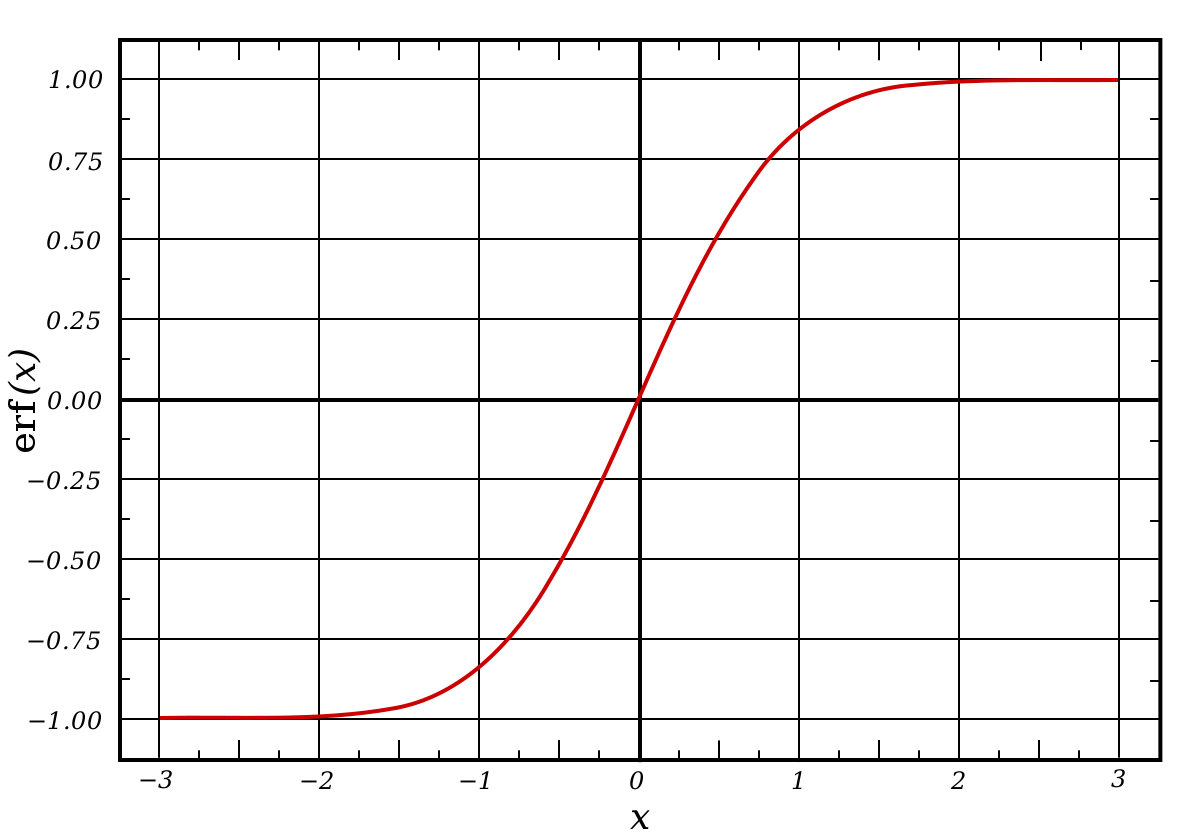
\includegraphics[scale=0.3]{images/error_function.png}
    \caption{Error function}
    \label{figure:error_function}
\end{figure}

\subsubsection{Overall Equipment Effectiveness}
The \textbf{O}verall \textbf{E}quipment \textbf{E}ffectiveness, OEE, is
basically a measurement of how effective a given production line is. It
identifies what percentage of the manufacturing time that is truly productive.
The formula for the OEE can be seen in equation 
\begin{equation} \label{eq:2}
    OEE = \frac{Good Count * Ideal Cycle Time}{Planned Produciton Time}
\end{equation}

Where \textit{GoodCount} is the amount of acceptable products produced and
\textit{IdeaCycleTime} is the theoretical minimum time to produce a single
product.

% Maybe delete the following
The OEE can also be found using the formula
\[
    OEE = Availability * Performance * Quality
\]

Where \(Availability = \frac{Run Time}{Planned Production Time}\),
\(Performance = \frac{Idea Cycle Time * Total Count}{Run Time}\) and
\(Quality = \frac{Good Count}{Total Count}\) \\

The OEE is calculated after each batch has run since the amount of acceptable
products is needed.

\subsection{Methods}
To keep track of the group work, the Scrum framework, with a few buts, is used.
Scrum consists of multiple artefacts and ceremonies, and in this project product
roadmap, Scrum meetings, product and sprint backlogs and burndown charts will
be used. Each sprint will have a duration of two weeks and the issues for the
sprint backlog will be chosen at the beginning of each sprint, at the Scrum
meeting. The Scrum meeting will take place each Friday and will be a mixture of
sprint planning, daily Scrum, and sprint review. To manage Scrum, ZenHub, a
management solution that can be integrated with GitHub, is used. On ZenHub the
group will create the roadmap, that acts as a schedule for the project and
board, which is where the issues will be handled. A burndown chart for each
sprint is automatically generated and kept up to date by ZenHub. The board will
consist of five columns, as seen below.

\begin{table}[H]
    \begin{tabularx}{\textwidth}{|>{\RaggedRight}X|>{\RaggedRight}X|>{\RaggedRight}X|>{\RaggedRight}X|>{\RaggedRight}X|>{\RaggedRight}X|>{\RaggedRight}X|}
        \hline                             
        \textbf{Product Backlog} & \textbf{Sprint Backlog} & \textbf{In Progress} & \textbf{Review/QA} & \textbf{Closed} \\
        \hline
        Issues & Issues for the given sprint & Issues that is currently being worked on & Issues that are pending (or in) review & Approved issues that have been merged    \\
        \hline
    \end{tabularx}
    \caption{Methods} 
    \label{table:Methods}
\end{table} 